\section{Алгоритм SIFT}

\textbf{Scale-invariant feature transform} (SIFT) - алгоритм компьютерного зрения для выделения ключевых точек и их дескрипторов. Алгоритм был разработан в Университете Британской Колумбии (Ванкувер, Канада) и опубликован Дэвидом Лоу (\textit{David G. Lowe}) в 1999 году \hyperref[itm:lowe]{[\ref{itm:lowe}]}. Применяется в следующих задачах: распознавание объектов, позиционирование и навигация роботов, склеивание изображений (построение панорамных снимков), 3D моделирование, распознавание жестов, трекинг видео (сопоставление перемещения).

\subsection{Удаление шумов}

Перед первым этапом алгоритма часто производится предварительная обработка изображения в целях улучшения его качества для последующего анализа. Например, на фотографиях с камер возможно появление шумов. Чтобы их устранить используют гауссовское размытие с маленьким радиусом или медианные фильтры, которые, работая с цифровым сигналом изображения подавляют шумовые частоты.

Фильтрация происходит следующим образом: каждый пиксель заменяется средним взвешенным значением в своей локальной окрестности. Веса, с которыми берутся значения каждого пикселя из локальной окресности составляют \textit{ядро фильтра}. Операция применения фильтра с ядром $g$ к изображению $f$ называется \textit{свёрткой}, обозначается как $f * g$ и вычисляется по формуле:
\begin{equation}
    (f * g)[m, n] = \sum_{k, l} f[m - k, n - l] * g[k, l]
\end{equation}

В фильтре Гаусса коэффициенты ядра распределены по нормальному двумерному распределению. Параметрами такого фильтра является коэффициент дисперсии $\sigma$ и размер ядра фильтра $r$. Обычно размер полагается равным $3\sigma$. Является низкочастотным фильтром: то есть пропускает только низкие частоты и подавляет высокие. С помощью фильтра Гаусса достигается эффект расфокусировки изображения.

Существует вид шумов, называемых \quotes{соль и перец} - случайные чёрные и белые пиксели на изображении. Для этого вида шума Гауссов фильтр будет работать плохо, так как он просто заменит белые пиксели на средние серые. В таких случаях используют \textit{медианный фильтр}. Он работает следующим образом: Все значения яркости пикселей из локальной окрестности раскладываются в ряд, сортируются и в качестве результирующего значения выибарется медиана. За счёт этого достигается устойчивось к одиночным выбросам (которыми и являются шумы \quotes{соль и перец}).

\subsection{Извлечение ключевых точек}

SIFT, также называемый методом Лоу (по имени автора), трансформирует исходное изображение в большую коллекцию особых векторов, каждый из которых инвариантен к основным изменениям изображения. Представим что у нас есть два изображения одного и того же объекта, но с большой разницей в масштабе (Рисунок \ref{fig:scale}). Вместо того, чтобы извлекать особенности на различных масштабах и потом сопоставлять их между собой, метод SIFT предлагает гораздо более эффективный способ: найти функцию от области изображения, такую, что для областей изображающих один и тот же объект, даже в разных масштабах, будет возвращать одинаковые значения.

\begin{figure}[h]
    \centering
    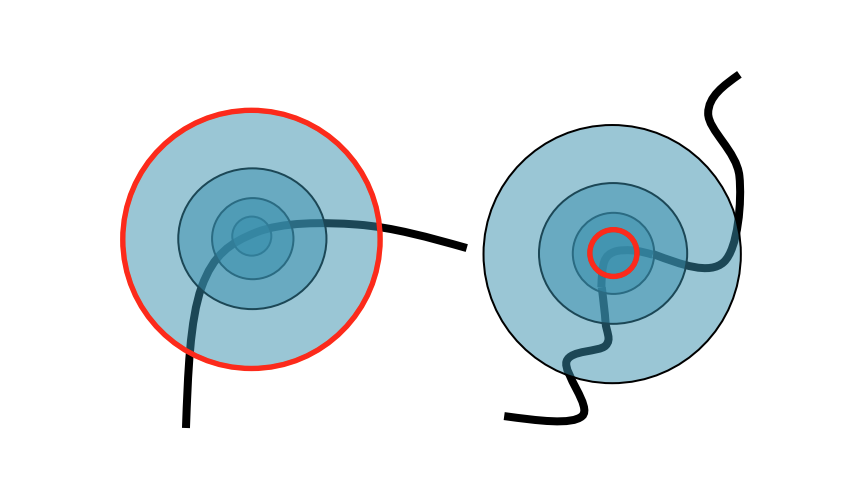
\includegraphics[width=0.6\textwidth]{features-scale.png}
    \caption{Красным цветом обведены области одного масштаба}
    \label{fig:scale}
\end{figure}


Основополагающим моментом в нахождении особых точек является построение пирамиды гауссианов (\textbf{Gaussian}) и разностей гауссианов (\textbf{Difference of Gaussian, DoG}).

Гауссианом (или изображением, размытым гауссовым фильтром) является изображение:
\begin{equation} \label{eq:1}
    L(x,y,\sigma) = G(x,y,\sigma) * I(x,y)
\end{equation}

В уравнении (\ref{eq:1}): $L$ — значение гауссиана в точке с координатами $(x,y)$, а $\sigma$ — радиус размытия. $G$ — гауссово ядро, $I$ — значение исходного изображения, $*$ — операция свертки.

Разностью гауссианов называют изображение, полученное путем попиксельного вычитания одного гауссиана исходного изображения из гауссиана с другим радиусом размытия:
\begin{equation} \label{eq:2}
    D(x,y,\sigma) = (G(x,y,k\sigma)-G(x,y,\sigma)) * I(x,y) = L(x,y,k\sigma) - L(x,y,\sigma)
\end{equation}

Таким образом, с помощью (\ref{eq:2}), мы получаем набор изображений, являющихся исходным изображением взятым в разных масштабах. Извлечение ключевых точек, таких что они являются неизменными на всех изображениях из этого набора будет гарантировать инвариантность относительно сдвига, поворота и изменения размера изображения. Для этого строится пирамида гауссианов (Рисунок \ref{fig:dog1}): весь набор масштабированных изображений разбивается на некоторые участки - октавы и при переходе от одной октавы к другой размеры изображения уменьшаются вдвое. После этого строится пирамида разностей гауссианов, состоящая из разностей соседних изображений в пирамиде гауссианов.

\begin{figure}[h]
    \centering
    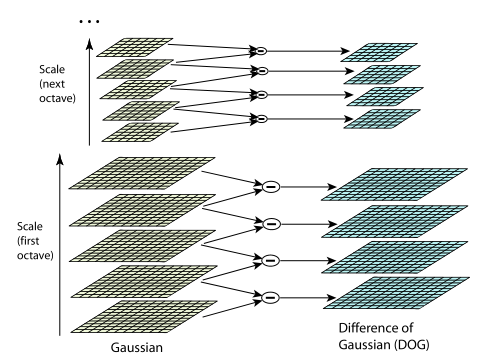
\includegraphics[width=0.6\textwidth]{dog.png}
    \caption{Пирамида гаусианнов}
    \label{fig:dog1}
\end{figure}

После построения пирамиды разностей гауссианов по всем точкам в пирамиде ищутся локальные экстремумы. Если точка больше (меньше) всех своих 26 соседей (Рисунок \ref{fig:dog2}) в пирамиде разностей, то она считается ключевой, а масштаб изображения на котором она вычислена берётся как основной.

\begin{figure}[h]
    \centering
    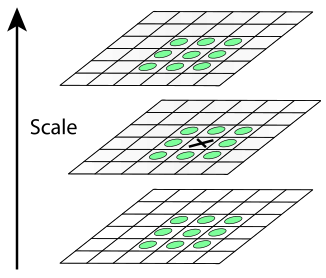
\includegraphics[width=0.5\textwidth]{dog2.png}
    \caption{Локальный экстремум в пирамиде Гауссианов}
    \label{fig:dog2}
\end{figure}

Направление особой точки вычисляется на изображении из пирамиды гауссианов в масштабе, полученном на предыдущем шаге. Ориентация ключевой точки - суммарное направление градиентов точек, находящихся в  $\sigma$-окрестности особой точки. Каждая точка окрестности влияет на итоговое направление. Вся особая область поворачивается так, чтобы доминантное направление градиента было направлено в одном направлении для всех точек, например вверх. Величина и направление градиента в точке $(x,y)$ вычисляются по формулам (\ref{eq:3}) и (\ref{eq:4}) соответственно.

\begin{equation} \label{eq:3}
    m(x,y)=\sqrt{(L(x+1,y) - L(x-1,y))^2 + (L(x,y+1) - L(x,y-1))^2}
\end{equation}

\begin{equation} \label{eq:4}
    \theta(x,y)=\arctan{\left(\frac{L(x,y+1) - L(x,y-1)}{L(x+1,y) - L(x-1,y)}\right)}
\end{equation}

Таким образом для исходных изображений разных размеров мы получили ключевые точки (и небольшую область возле них) одного и того же размера - это и даёт инвариантность относительно масштабирования. А с помощью ориентации особой точки достигается инвариантность относительно поворота.

\subsection{Извлечение дескрипторов}

Как уже говорилось ранее, дескриптор должен уникально описывать ключевую точку. В общем случае это может быть любой объект, который будет выполнять данные функции: быть удобным для сравнения и являться инвариантным относительно преобразований исходного изображения.

В алгоритме SIFT дескриптор представляется как вектор, содержащий информацию об окрестности ключевой точки. Дескриптор вычисляется на том же гауссиане, на котом получен оптимальный размер особой точки. Для достижения инвариантности относительно поворота изображения перед вычислением всю область ключевой точки поворачивают на угол направления ключевой точки, который был найден на предыдущем шаге алгоритма.

\begin{figure}[h]
    \centering
    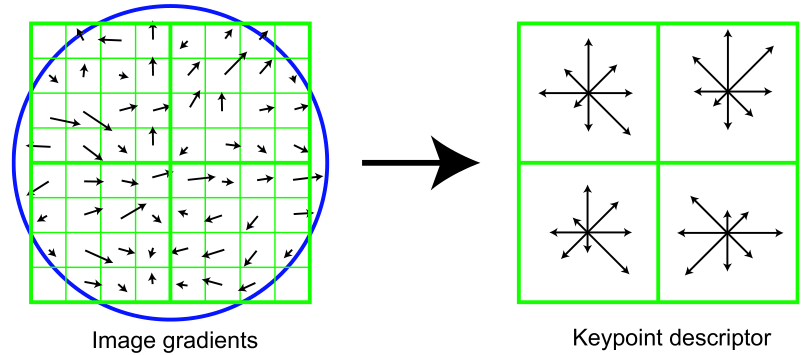
\includegraphics[width=0.8\textwidth]{desc.png}
    \caption{Получение дескриптора}
    \label{fig:desc}
\end{figure}

На Рисунке \ref{fig:desc} показана окрестность ключевой точки (слева) и построенный для неё дескриптор, состоящий из гистограмм направлений градиентов (справа). Стрелочками в центре каждого пикселя в $\sigma$-окрестности обозначен градиент этого пикселя. Как видно на правой стороне изображения, дескриптор имеет размерность 2x2x8 (количество регионов по горизонтали, количество регионов по вертикали, количество компонент гистограммы этих регионов). Гистограмма для каждого региона является суммарным значением градиентов пикселей, входящих в $\sigma$-окрестность ($8$ штук).

Все полученные гистограммы и составляют итоговый дескриптор ключевой точки. В конце дескриптор нормализуется - все компоненты делятся на максимальное значение - в итоге каждая компонента находится в диапазоне $[0,1]$. Далее всем компонентам, значение которых больше $0.2$, присваивается значение $0.2$, а после этого дескриптор нормализуется ещё раз.

Как говорилось ранее, размер дескриптора равен 2x2x8 = $32$ компоненты, но на практике больше распространены и активнее используются дескрипторы размерности $128$ компонент (4x4x8).

Так как в качестве значений вектора дескриптора используются градиенты, это значит что он будет является инвариантным к изменению освещения, потому что это будет отражено в гистограмме.